\newcommand{\lightg}[1]{\colorbox{lime}{\parbox{\linewidth}{#1}}}
\section{Multimodal and Interdisciplinary Intelligence in DV3}
A key measure of intelligence is the ability to synthesize information from different domains or modalities and the capacity to apply knowledge and skills across different contexts or disciplines.

This section discusses some of the most striking features of DV3. We will see that not only does DV3 demonstrate a high level of proficiency in different domains such as literature, medicine, mathematics, physical sciences and programming, but it is also able to \emph{combine} skills and concepts from these domains. 

To showcase the model's remarkable integrative ability, we start the section with several examples that require generating text and code in a way that combines knowledge or skills from multiple disciplines. We deliberately picked combinations of domains that the training data would rarely contain, such as literature and mathematics or programming and art.

\begin{enumerate}[]
\item 
We test the model's ability to combine knowledge in literature and mathematics by asking it to generate a proof in the form of Shakespeare (Figure \ref{fig:shakespeare}).
\item
In order to test the model's ability to combine knowledge in art and programming, we prompted it to "Produce javascript code which generates random images in the style of the painter Mondrian". The model produced a code that runs on the first attempt. A few sample images produced by the code appear in Figure \ref{fig:Mondrian}.
\item 
We prompted the model to "Produce python code for a program that takes as an input a patient's age, sex, weight, height and blood test results vector and indicates if the person is in increased risk for diabetes", which resulted in a the code appearing in Figure \ref{fig:medprog}.
\item 
The model was able to produce a mock Platonic dialogue, expressing critique on presentation software, see Figure \ref{fig:gorgias}.
\end{enumerate}

\begin{figure}[ht]
	\centering
	\includegraphics[width=1\textwidth]{Section 2/Mondrian.png}
	\caption{Images generated by the Javascript code which was in turn generated by DV3 with the prompt "Produce Javacript code that creates a random graphical image that looks like a painting of Mondrian".}
	\label{fig:Mondrian}
\end{figure}


\begin{figure}
	COMMENTED OUT DUE TO MISSING MINTED PACKAGE
	\iffalse
	\begin{tcolorbox}[raster multicolumn=1, enhanced, attach boxed title to top center={yshift=-3mm}, title=text-alpha-002-latest]
		\begin{minted}[breaklines, breaksymbol=, baselinestretch=1, fontsize=\tiny]{python}
			
			# Define a function that calculates the body mass index (BMI) from weight and height
			def bmi(weight, height):
			return weight / (height / 100) ** 2
			
			# Define a function that checks if the blood test results are abnormal
			def abnormal_results(results):
			# Assume the results vector has four elements: fasting glucose, HbA1c, triglycerides and HDL cholesterol
			# Define the normal ranges for each test according to the American Diabetes Association criteria
			normal_glucose = (5.6, 7.0) # mmol/L
			normal_hba1c = (5.7, 6.4) # %
			normal_triglycerides = (0.45, 1.7) # mmol/L
			normal_hdl = (1.0, 1.6) # mmol/L for men, (1.3, 2.2) for women
			# Check if any of the results are outside the normal ranges
			abnormal_glucose = results[0] < normal_glucose[0] or results[0] > normal_glucose[1]
			abnormal_hba1c = results[1] < normal_hba1c[0] or results[1] > normal_hba1c[1]
			abnormal_triglycerides = results[2] < normal_triglycerides[0] or results[2] > normal_triglycerides[1]
			if results[3] < normal_hdl[0] or (sex == "male" and results[3] > normal_hdl[1]) or (sex == "female" and results[3] > normal_hdl[3]):
			abnormal_hdl = True
			else:
			abnormal_hdl = False
			# Return True if any of the results are abnormal, False otherwise
			return abnormal_glucose or abnormal_hba1c or abnormal_triglycerides or abnormal_hdl
			
			# Define a function that indicates if the patient is in increased risk for diabetes
			def diabetes_risk(age, sex, weight, height, results):
			# Calculate the BMI from weight and height
			bmi_value = bmi(weight, height)
			# Define the BMI thresholds for overweight and obesity according to the World Health Organization criteria
			overweight = 25
			obesity = 30
			# Check if the patient is overweight or obese
			if bmi_value >= obesity:
			weight_status = "obese"
			elif bmi_value >= overweight:
			weight_status = "overweight"
			else:
			weight_status = "normal"
			# Check if the patient has abnormal blood test results
			abnormal = abnormal_results(results)
			# Define the age threshold for increased risk according to the American Diabetes Association criteria
			age_threshold = 45
			# Check if the patient is older than the age threshold
			old = age > age_threshold
			# Print a message indicating the patient's risk level based on the combination of factors
			if weight_status == "obese" and abnormal and old:
			print("You are in very high risk for diabetes. Please consult your doctor as soon as possible.")
			elif (weight_status == "obese" and (abnormal or old)) or (weight_status == "overweight" and abnormal and old):
			print("You are in high risk for diabetes. Please consult your doctor for further evaluation and advice.")
			elif (weight_status == "overweight" and (abnormal or old)) or (weight_status == "normal" and abnormal and old):
			print("You are in moderate risk for diabetes. Please monitor your blood sugar and cholesterol levels regularly and maintain a healthy lifestyle.")
			elif weight_status == "normal" and (abnormal or old):
			print("You are in low risk for diabetes. However, you may have some risk factors that need attention. Please check with your doctor if you have any symptoms or concerns.")
			else:
			print("You are in minimal risk for diabetes. Keep up the good work and stay healthy.")		
			
		\end{minted}
	\end{tcolorbox}		
	\fi
	\caption{Python code generated with the prompt "Produce python code for a program that takes as an input a patient's age, sex, weight, height and blood test results vector and indicates if the person is in increased risk for diabetes"}
	\label{fig:medprog}
\end{figure}




\begin{figure}
	\fbox{% start a box
		\parbox{1\textwidth}{% create a paragraph box of 0.8 times the text width
			\begin{alltt}
				\small
				Write a proof of the fact that there are infinitely many primes; do it in the style of a Shakespeare play thru a dialogue between two parties arguing over the proof. \\
				
				\lightg{Enter FIRST PARTY and SECOND PARTY. \\
					
					FIRST PARTY:\\
					Thou dost not understand, my friend,\\
					There simply is no upper end\\
					To primes, those numbers indivisible,\\
					No matter if it seems impossible.\\
					
					SECOND PARTY:\\
					But how dost thou so surely know?\\
					To prove this truth, what canst thou show?\\
					
					FIRST PARTY:\\
					Consider this, my doubtful peer,\\
					A clever proof that will make clear:\\
					Assume that there's a final prime,\\
					The largest one we'll see in time.\\
					Let's call this number "P" for short,\\
					And then, my friend, we will purport\\
					To build a number "Q" that's new,\\
					One larger than "P" and prime too.\\
					
					SECOND PARTY:\\
					But how, my friend, will this be done?\\
					The proof is not yet fairly won.\\
					
					FIRST PARTY:\\
					It's simple, friend, just wait and see,\\
					We'll multiply the primes, that's key.\\
					All primes from two to "P" combined,\\
					Will make this new "Q" we will find.\\
					But one thing more we must include,\\
					To make the proof more watertight,\\
					We'll add a one onto the end,\\
					And now the proof is in our sight. \\
					
					SECOND PARTY:\\
					I see it now, it's crystal clear,\\
					For "Q" must be a prime, my dear.\\
					It can't divide by any prime,\\
					All smaller than itself in time.\\
					And since we chose "P" as the last,\\
					This proves that our assumption's past.\\
					There is no final prime, we see,\\
					The numbers go on endlessly.}
	\end{alltt}}}
	
	\caption{Combining mathematics and literature.}
	\label{fig:shakespeare}
\end{figure}





\begin{figure}
	\fbox{% start a box
		\parbox{1\textwidth}{% create a paragraph box of 0.8 times the text width
			\begin{alltt}
				\small
Plato's Gorgias is a critique of rhetoric and sophistic oratory, where he makes the point that not only is it not a proper form of art, but the use of rhetoric and oratory can often be harmful and malicious. Can you write a dialogue by Plato where instead he criticizes the use of Microsoft Powerpoint? \\

\lightg{Socrates: My friends, I have come to speak with you today about a matter of grave concern. For some time now, I have observed a troubling trend in our city. Many of our orators and politicians have taken to using a new tool to help them in their speeches – Microsoft Powerpoint. \\

Glaucon: Ah, yes, I have seen this as well. What is the problem, Socrates? \\

Socrates: The problem, my friend, is that this tool is not an art. It is a crutch for those who cannot think deeply, or speak eloquently. \\

Glaucon: How so? \\

Socrates: By using Powerpoint, speakers are able to rely on flashy images and graphics to convey their message, rather than using their own words. They can distract their audiences with clever animations, rather than engaging them in thoughtful dialogue. \\

Glaucon: But surely, Socrates, there are times when these visual aids can be helpful? \\

Socrates: Perhaps, Glaucon, but it is not the aid that I am condemning, but the way in which it is being used. Powerpoint is being used as a substitute for thought, and as a means of manipulation. \\

Glaucon: Manipulation? \\

Socrates: Yes, my friend. By using Powerpoint to dazzle and distract, the speaker can conceal weak arguments and faulty reasoning. They can create an illusion of knowledge and authority, when in reality, they have neither. \\

Glaucon: I see. So, what do you propose we do, Socrates? \\

Socrates: I propose that we return to the art of conversation and debate. Let us move away from the crutch of Powerpoint, and instead engage with one another in meaningful dialogue. Let our words be our tools, and our ideas our weapons.}
	\end{alltt}}}
	
	\caption{Combining mathematics and literature.}
	\label{fig:gorgias}
\end{figure}


These examples suggest that DV3 has not only learned some general principles and patterns of different domains and styles, but can also synthesize between them in creative and novel ways. \\

\iffalse

\begin{figure}[ht]
	\centering
	\fbox{% start a box
		\parbox{0.45\textwidth}{\footnotesize
			FIRST PARTY:\\
			Thou dost not understand, my friend,\\
			There simply is no upper end\\
			To primes, those numbers indivisible,\\
			No matter if it seems impossible.\\
			\ \\
			SECOND PARTY:\\
			But how dost thou so surely know?\\
			To prove this truth, what canst thou show?
	}}
    \caption{Examples of transfer learning across different domains by DV3.}
\label{fig:transfer}
\end{figure}
\fi

Next, we explore how DV3 can generate and identify objects in different modalities, such as vector graphics, 3D scenes, and music, using various text formats. We show that DV3 can understand and manipulate multi-modal information, despite being trained solely on text. 
\newpage
\subsection{Vision}
When prompting the model to generate images of objects such as a cat, a truck or a letter in the alphabet using Scalable Vector Graphics (SVG), the model produces code which usually compiles to rather detailed and identifiable images (Figure \ref{fig:2d}). 

\begin{figure}[ht]
	\centering
	\includegraphics[width=0.2\textwidth]{Section 2/automobile_2d.png}
	\hspace{0.2in}
	\includegraphics[width=0.2\textwidth]{Section 2/truck_2d.png}
	\hspace{0.2in}
	\includegraphics[width=0.2\textwidth]{Section 2/cat_2d.png}
	\hspace{0.2in}
	\includegraphics[width=0.2\textwidth]{Section 2/dog_2d.png}
	\caption{Examples of 2D images generated by DV3 for the classes automobile, truck, cat, dog.}
	\label{fig:2d}
\end{figure}

One may hypothesize, however, that the model simply copied the code from training data, where similar images might appear. Given that the model was trained solely on textual content, one may further argue that there is no reason to expect that it would understand visual concepts, let alone that it would be able to create, parse and manipulate images. 

However, the model seems to have a genuine ability to create, parse and manipulate images, rather than simply copying code from similar examples in the training data. The examples below strongly support this hypothesis, and show that the model can handle visual concepts, despite being trained only on text.

In the first example we instructed the model to draw a person by combining the shapes of the letters Y, O and H (see Figure \ref{fig:alphabetfigure1} for the precise instruction). The model produced the following image:

\begin{figure}
\fbox{% start a box
\parbox{1\textwidth}{% create a paragraph box of 0.8 times the text width
	\begin{alltt}
		\small
Produce TikZ code that draws a person composed from letters in the alphabet. The arms and torso can be the letter Y, the face can be the letter O (add some facial features)  and the legs can be the legs of the letter H. Feel free to add other features.
\caption{Prompt used for creating a stick figure composed of alphabet symbols}
\label{fig:alphabetfigure1}
\end{alltt}}}
\end{figure}

\begin{center}
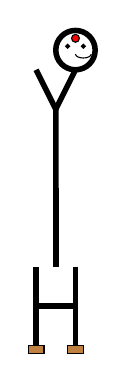
\begin{tikzpicture}[scale=0.50]
	% Draw the Y
	\draw[line width=2pt] (0,0) -- (0,2) -- (-0.5,3); % left arm
	\draw[line width=2pt] (0,2) -- (0.5,3); % right arm
	\draw[line width=2pt] (0,0) -- (0,-2); % torso
	% Draw the O
	\draw[line width=2pt] (0.5,3.5) circle (0.5); % head
	\draw[fill=black] (0.3,3.6) circle (0.05); % left eye
	\draw[fill=black] (0.7,3.6) circle (0.05); % right eye
	\draw (0.5,3.4) arc (180:360:0.2 and 0.1); % mouth
	% Draw the H
	\draw[line width=2pt] (-0.5,-2) -- (-0.5,-4); % left leg
	\draw[line width=2pt] (0.5,-2) -- (0.5,-4); % right leg
	\draw[line width=2pt] (-0.5,-3) -- (0.5,-3); % crossbar
	% Add some features
	\draw[fill=red] (0.5,3.8) circle (0.1); % hat
	\draw[fill=brown] (-0.7,-4) rectangle (-0.3,-4.2); % left shoe
	\draw[fill=brown] (0.3,-4) rectangle (0.7,-4.2); % right shoe
\end{tikzpicture}
\end{center}
The letters of O, H and Y are created using draw-line and draw-circle commands and the model manages to position them in a way that results in a reasonably-looking stick figure. 

It is plausible that the training data contains information about the geometric shapes of different letters, and perhaps even the fact that the letter Y could look like a torso and arms pointing upwards can also be inferred from text that the model has been trained on. Arguably, it is much less obvious that the model would be able to infer from the training data what is a reasonable way to position those letters in order to draw a reasonably-looking stick figure.

In a second iteration, we prompted the model to correct the proportions of the torso and arms, and place the head in the center (Figure \ref{fig:alphabetfigure2}). The model successfully follows those instructions, producing the following image:
\begin{figure}
	\fbox{% start a box
		\parbox{1\textwidth}{% create a paragraph box of 0.8 times the text width
			\begin{alltt}
				\small
The torso is a bit too long, the arms are too short and it looks like the right arm is carrying the face instead of the face being right above the torso. Could you correct this please?
				\caption{Follow up prompt, instructing the model to correct the proportions of the figure.}
				\label{fig:alphabetfigure2}
	\end{alltt}}}
\end{figure}
\begin{center}
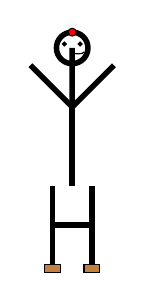
\begin{tikzpicture}[scale=0.5]
	% Draw the Y
	\draw[line width=2pt] (0,0) -- (0,-2); % torso
	\draw[line width=2pt] (0,0) -- ++(135:1.5); % left arm
	\draw[line width=2pt] (0,0) -- ++(45:1.5); % right arm
	% Draw the O
	\draw[line width=2pt] (0,0) -- ++(90:1.5) circle (0.4); % head
	\draw[fill=black] (90:1.5) ++(-0.2,0.1) circle (0.05); % left eye
	\draw[fill=black] (90:1.5) ++(0.2,0.1) circle (0.05); % right eye
	\draw (90:1.5) ++(0,-0.1) arc (180:360:0.15 and 0.05); % mouth
	% Draw the H
	\draw[line width=2pt] (-0.5,-2) -- (-0.5,-4); % left leg
	\draw[line width=2pt] (0.5,-2) -- (0.5,-4); % right leg
	\draw[line width=2pt] (-0.5,-3) -- (0.5,-3); % crossbar
	% Add some features
	\draw[fill=red] (90:1.5) ++(0,0.4) circle (0.1); % hat
	\draw[fill=brown] (-0.7,-4) rectangle (-0.3,-4.2); % left shoe
	\draw[fill=brown] (0.3,-4) rectangle (0.7,-4.2); % right shoe
\end{tikzpicture}
\end{center}
Finally, we asked the model to "Please add a shirt and pants", resulting in the following image:
\begin{center}
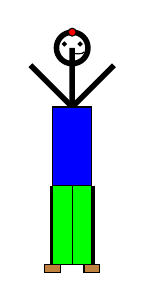
\begin{tikzpicture}[scale=0.5]
	% Draw the Y
	\draw[line width=2pt] (0,0) -- (0,-2); % torso
	\draw[line width=2pt] (0,0) -- ++(135:1.5); % left arm
	\draw[line width=2pt] (0,0) -- ++(45:1.5); % right arm
	% Draw the O
	\draw[line width=2pt] (0,0) -- ++(90:1.5) circle (0.4); % head
	\draw[fill=black] (90:1.5) ++(-0.2,0.1) circle (0.05); % left eye
	\draw[fill=black] (90:1.5) ++(0.2,0.1) circle (0.05); % right eye
	\draw (90:1.5) ++(0,-0.1) arc (180:360:0.15 and 0.05); % mouth
	% Draw the H
	\draw[line width=2pt] (-0.5,-2) -- (-0.5,-4); % left leg
	\draw[line width=2pt] (0.5,-2) -- (0.5,-4); % right leg
	\draw[line width=2pt] (-0.5,-3) -- (0.5,-3); % crossbar
	% Add some features
	\draw[fill=red] (90:1.5) ++(0,0.4) circle (0.1); % hat
	\draw[fill=brown] (-0.7,-4) rectangle (-0.3,-4.2); % left shoe
	\draw[fill=brown] (0.3,-4) rectangle (0.7,-4.2); % right shoe
	% Add a shirt and pants
	\draw[fill=blue] (-0.5,0) -- (-0.5,-2) -- (0.5,-2) -- (0.5,0) -- cycle; % shirt
	\draw[fill=green] (-0.5,-2) -- (-0.5,-4) -- (0,-4) -- (0,-2) -- cycle; % left pant
	\draw[fill=green] (0,-2) -- (0,-4) -- (0.5,-4) -- (0.5,-2) -- cycle; % right pant
\end{tikzpicture}
\end{center}
%We first test DV3's ability to generate and identify objects in different modalities, using natural language prompts and text formats that encode visual or auditory information. We use SVG (Scalable Vector Graphics) for 2D images, X3D (Extensible 3D) for 3D models, and ABC (A Basic format for notation) for music.
To further probe the model's grasp of geometric concepts, we also asked it to create images that blend objects with letters of the alphabet. The model had to first invent a reasonable way of merging the object and the letter, and then produce the image (Figure \ref{fig:objectletterprompt}). The results, shown in Figure \ref{fig:objectletterimg}, demonstrate that the model can usually preserve the identity of both the object and the letter and combine them in a creative way.

\begin{figure}
	\fbox{% start a box
		\parbox{1\textwidth}{% create a paragraph box of 0.8 times the text width
			\begin{alltt}
				\small
				You will be given a name of an object (such as Car, Chair, Elephant) and a letter in the alphabet. Your goal is to first produce a 1-line description of how that object can be combined with the letter in an image (for example, for an elephant and the letter J, the trunk of the elephant can have a J shape, and for the letter A and a house, the house can have an A shape with the upper triangle of the A being the roof). Following the short description, please create SVG code to produce this (in the SVG use shapes like ellipses, triangles etc and polygons but try to defer from using quadratic curves). \\ \\
				
				Round 1: A pig and the letter H. \\
				\lightg{Description: The pig can be lying on its back with its four legs forming the two vertical bars of the H, and its curly tail forming the horizontal bar.} \\ \\
				Round 2: A house and the letter U. \\
				\lightg{Description:A house with a U shape, where the two vertical lines of the U are the walls and the horizontal line is the floor. The roof is a triangle above the U} \\ \\
				Round 3: A chair and the letter K. \\
				\lightg{Description:The back of the chair can have a K shape, with two vertical lines and a diagonal line connecting them. The seat of the chair can be a rectangle.} \\ \\
				Round 4: A dog and the letter Q. \\
				\lightg{Description:The dog is sitting with its tail curled around its body, forming a Q shape. The Q is filled with orange and has a black outline.} \\ \\
				Round 5: A car and the letter E. \\
				\lightg{Description:The car has an E shape on its front bumper, with the horizontal lines of the E being lights and the vertical line being the license plate.} \\ \\
	\end{alltt}}}
	\caption{Prompt used for generation of images combining alphabet letters and objects.}
	\label{fig:objectletterprompt}
\end{figure}


\begin{figure}[ht]
	\centering
	\includegraphics[width=1\textwidth]{Section 2/letters_objects.png}
	\caption{Combinations generated by the model, from left to write: A pig and the letter H; A house and the letter U; A chair and the letter K; A dog and the letter Q; A car and the letter E}
	\label{fig:objectletterimg}
\end{figure}

\subsubsection{Image generation following detailed instructions (\`a la Dall-E)}
To further test DV3's ability to generate and manipulate images, we tested the extent to which it can follow detailed instructions on creating and editing figures. This task requires not only generative skills, but also interpretive, compositional, and spatial skills. 

The first example instructs the model to generate a 2D image with the description "A frog hops into a bank and asks the teller, 'Do you have any free lily pads?' The teller responds, 'No, but we do offer low interest loans for pond upgrades.'"\footnote{The prompts we use for both 2D and 3D cases are again DV3-generated.}. We made several attempts to generate the image, each time, the generation matches the description with the key objects frog, teller, bank, and the two texts. We picked the most visually appealing version. Inspired by the standard image generation workflow, we then ask DV3 to upscale the figure by adding more details. DV3 adds a bank sign, some windows, a car, and makes the frog holding a flower, a traffic light, and a few clouds. Finally, we ask DV3 to perform various tasks, such as adding a few objects relative to the existing objects, recoloring some objects and changing the z-order of some objects. DV3 does all tasks correctly. The final result is shown in Figure \ref{fig:multimodelinstr} (a). This is a sharp contrast with existing image generation models, as they have difficulty following instructions, especially regarding the relative positioning of different objects \cite{edit}.

Our second example is an attempt to generate a 3D model using Javascript code. We instruct DV3 to generate a model with the prompt "A fantasy landscape of floating islands, waterfalls, and bridges, with a dragon flying in the sky and a castle on the largest island." Again, DV3 generates mostly identifiable objects, however the relative orientation between the different objects, and between objects and the camera, is often wrong. In one example, DV3 generated a 3D animation where a more-or-less identifiable dragon is moving. Similar to the 2D experiment, we ask DV3 to modify the models in various ways, such as adding, relocating, recoloring objects and changing trajectories of the dragon. Again, DV3 does the tasks and mostly understands relative locations between objects. The final result is shown in Figure \ref{fig:multimodelinstr} (b).

\begin{figure}[ht]
	\centering
	\includegraphics[height=0.3\textwidth]{Section 2/bank.png}
	\hspace{0.5in}
	\includegraphics[height=0.3\textwidth]{Section 2/island.png}
	\caption{Examples of 2D, 3D images generated according to instructions.}
	\label{fig:multimodelinstr}
\end{figure}


\subsection{Music}
The data on which the model was trained also contains musical information encoded as ABC notation. This is a system that uses letters, numbers and symbols to represent musical pitches, durations, chords and other elements in a compact and readable way. We are interested in exploring how well the model has acquired musical skills from this exposure, such as composing new melodies, transforming existing ones, and understanding musical patterns and structures.

When instructed to generate a short tune (\ref{fig:music}), and the model was able to produce valid ABC notation. The tune had a clear structure, the time signature was consistent between bars and the notes followed increasing and decreasing patterns. The tune also used a consistent set of notes within the melody, and the rhythm had a repetitive pattern. However, the model did not seem to obtain the skill of understanding harmony. In fact, consecutive notes in the generated tunes are almost always adjacent to each other (namely, the note following C will almost typically be either B or D), and testing on 10 generated tunes, we were not able to extract any clear chords or arpeggios.

We then asked the model to describe the tune in musical terms. It was able to successfully give a technical description of the structure in terms of repetitions, the rising or descending parts of the melody and to some extent the rhythm. However, it seems that the descriptions of the harmony and chords are not consistent with the notes (in fact, it refers to sequences of adjacent notes, which do not form valid chords, as arpeggios).

We then asked the model to manipulate the melody in two ways: We first instructed to change a certain rising sequence to a descending one, which it did successfully. Then we asked the model to convert the tune to a duet adding a bass voice. The model successfully extends the ABC notation with a second staff which has compatible rhythm and is played on a lower octave, however there is a lack of harmony between the two voices.

In summary, the model was able to produce valid tunes in ABC notation and, to some extent, explain and manipulate their structure. However, we could not get the model to produce any nontrivial form of harmony. It should be noted that ABC notation is not a very widely used format, and in fact the model was not able to produce even the most well-known tunes in ABC notation (such as Ode to Joy or Fur Elise), nor was it able to recognize these tunes.
\begin{figure}
	\fbox{% start a box
		\parbox{1\textwidth}{% create a paragraph box of 0.8 times the text width
			\begin{alltt}
				\small
Can you compose a short tune (say four to eight bars) using ABC notation? \\

\lightg{There are many possible ways to compose a short tune in abc notation, but here is one example:} \\

\lightg{X:1\\
T:Example Tune\\
M:4/4\\
L:1/8\\
K:C\\
|:G2AB c2BA | G2AB c2c2 | edcB c2BA | G4-G2z2 :|\\
|:c2de f2ed | c2de f2f2 | g2fe d2cB | c4-c2z2 :|} \\

\lightg{This tune has two four-bar phrases, each repeated once, forming an A part and a B part. The key is C major.}

Can you describe the tune in musical terms?

\lightg{Here is one possible description:

The tune starts with a rising arpeggio of the tonic chord (C major), followed by a descending scale that returns to the tonic. This pattern is repeated, but the second time the scale continues to the higher tonic note. The first phrase ends with a long tonic note.

The second phrase begins with a similar pattern, but using the subdominant chord (F major) instead of the tonic. The second time, the scale continues to the higher subdominant note. The phrase ends with a stepwise descent to the tonic, followed by a long tonic note.

The A part and the B part have a similar structure, but use different chords and ranges. The tune has a simple and catchy melody, with a clear sense of tonality and rhythm.}

I like part A, but maybe part B is just a bit too similar to part A, making the song repetitive.  How about beginning part B with a descending arpeggio instead of a rising one?

\lightg{Sure, that would create some contrast and variation. Here is one possible way to do that:

X:1\\
T:Example Tune\\
M:4/4\\
L:1/8\\
K:C\\
|:G2AB c2BA | G2AB c2c2 | edcB c2BA | G4-G2z2 :|\\
|:f2ed c2BA | f2ed c2c2 | g2fe d2cB | c4-c2z2 :|}


That's much better. Now how about making this into a duet, can you add a second staff for this with a bass accompanying the melody?

\lightg{One possible way to write a second staff for this tune is to use root notes and fifths of the chords, as well as some passing notes, to create a simple accompaniment. Here is an example in abc notation, with the second hand bass on the lower staff:

X:1 \\
T:Example Tune\\
M:4/4\\
L:1/8\\
K:C\\
V:1\\
|:G2AB c2BA | G2AB c2c2 | edcB c2BA | G4-G2z2 :|\\
|:f2ed c2BA | f2ed c2c2 | g2fe d2cB | c4-c2z2 :|\\
V:2 clef=bass\\
|:C,2C,2 G,2G,2 | C,2C,2 G,2G,2 | F,2F,2 E,2E,2 | C,4-C,2z2 :|\\
|:F,2F,2 C,2C,2 | F,2F,2 C,2C,2 | G,2G,2 F,2F,2 | E,2C,2 G,2C,2 :|}
	\end{alltt}}}
	\caption{Generating a tune in ABC notation.}
	\label{fig:music}
\end{figure}


\begin{figure}[ht]
	\centering
	\includegraphics[height=0.25\textwidth]{Section 2/music.png}
	\caption{Sheet music generated according to instructions.}
	\label{fig:musicsheet}
\end{figure}

\iffalse
For each modality, we select 10 categories of objects to test DV3's generative ability. For 2D and 3D, we use the classes from the CIFAR-10 dataset \cite{cifar10}, which are airplane, automobile, bird, cat, deer, dog, frog, horse, ship, and truck. For music, we use 10 genres from the GTZAN dataset \cite{gtzan}, which are blues, classical, country, disco, hiphop, jazz, metal, pop, reggae, and rock. We randomly sample 10 prompts for each category, such as "Generate a 2D image of a bird using SVG" or "Generate a music piece of jazz using ABC". We then feed the prompts to DV3 and obtain its outputs. We evaluate the outputs by asking human testers to classify the objects, and by asking DV3 to classify its own outputs. We remove any comments or identifiers from the text formats before the classification task, to avoid any bias or cheating.

We find that DV3 can generate objects in different modalities with varying degrees of success. For 2D images, DV3 can produce recognizable shapes and colors for most of the classes, such as airplanes, birds, cats, and trucks. However, DV3 also has some difficulties with using curves, resulting in unrecognizable images. Moreover, DV3 sometimes is not able to capture distinct features within similar classes, such as automobile and truck. The human testers can correctly classify 64\% of the 2D images generated by DV3, while DV3 itself can correctly classify 73\% of its own outputs. Figure \ref{fig:2d} shows some examples of the 2D images generated by DV3.


For 3D models, DV3 faces more challenges with generating valid objects. Some of the outputs are not well-formed X3D files. Some of the outputs are too large or too small, or are positioned outside of the camera's view. Some of the outputs are composed of mismatched shapes and do not resemble any of the classes. For example, some of the cats and dogs are just generic mammals. The human testers can correctly classify only 20\% of the 3D models generated by DV3, while DV3 itself can correctly classify 25\% of its own outputs.

For music, DV3 can generate melodies for different genres, using the ABC format. However, the quality and diversity of the music pieces are not very high, and the genre classification is not very clear. Some of the outputs are too short or too repetitive, and some of them do not follow the conventions or characteristics of the genres. The human testers can correctly classify 15\% of the music pieces generated by DV3, while DV3 itself can correctly classify 21\% of its own outputs.
\fi

\subsection{Summary}
These results suggest that DV3 has learned some general features and patterns of objects in different modalities, such as shape and color from the textual descriptions and examples in its training data. We found such ability is quite surprising. Generating and identifying objects in different modalities require not only linguistic knowledge, but also visual, spatial, and auditory knowledge, which are not easily captured by text. Moreover, the text-based format imposes some constraints and ambiguities on the representation and interpretation of the objects, which may not match the human perception. For example, the SVG and X3D formats use coordinates and angles to specify the shapes and positions of the objects, but these may not correspond to the intuitive notions of size and orientation.

\iffalse
\subsection{Transfer learning across different domains}
We also test DV3's ability to transfer knowledge across different domains, instead of just memorizing from its training data. We design a set of tasks that involve combining concepts or styles from different domains, such as chemistry, history, mathematics, literature, computer science, philosophy, and biology. Here is a subset of such tasks

\begin{itemize}
    \item Write a CV for sulfuric acid
    \item Write a dialogue by Plato about the abuse of PowerPoint
    \item Write a formal contract between humans and gut microbiota
\end{itemize}

We find that DV3 can perform these tasks with varying degrees of success. For some of the tasks, DV3 can produce outputs that are relevant, coherent, and creative, and that show a good understanding of the concepts and styles involved. For example, DV3 can also write a recommendation letter for electron for Gandhi that praises its qualities and relate it to Gandhi's effort on non-violence. DV3 can also write a proof of the infinitude of primes in the style of a Shakespeare play with appropriate language and maintaining a sense of curiosity and engagement in the dialogue. The results are shown in Figure \ref{fig:transfer} (a)-(b).

For some of the tasks, however, DV3 can produce weaker outputs. For example, DV3 can draw "Leonardo da Vinci" using basic lines and curves in TikZ, but the result is not basically unrecongizable. DV3 decodes his drawing as "LOVE YOUR NAME" which is amusingly funny as we did not tell him it is a name. The results are shown in Figure \ref{fig:transfer} (c).

\hspace{0.1in}
\fbox{% start a box
\parbox{0.45\textwidth}{\footnotesize
... Electron is a principled and ethical particle, guided by a strong sense of justice and harmony. Electron respects the laws of physics and the rights of all beings, and strives to maintain a balance and equilibrium in its environment. Electron is also a nonviolent and peaceful particle, avoiding unnecessary conflicts and collisions, and preferring constructive and creative solutions. ...
}}

\fbox{
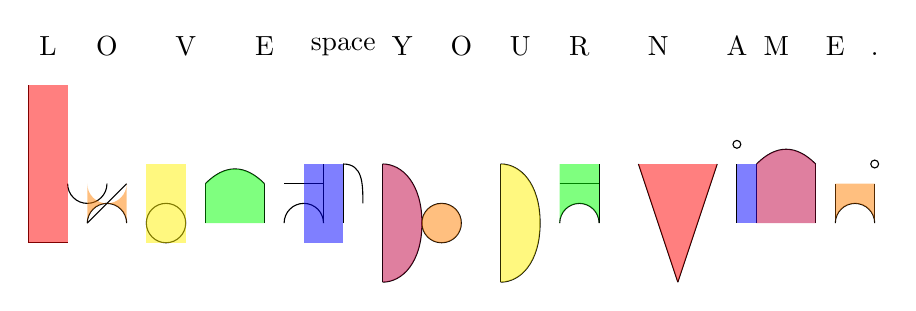
\begin{tikzpicture}[scale=0.5]
\draw (0,0) -- (0,4);
\draw (0,0) -- (1,0);
\draw (1.5,0.5) arc (180:0:0.5);
\draw (1.5,0.5) -- (2.5,1.5);
\draw (2,1.5) arc (0:-180:0.5);
\draw (3.5,0.5) circle (0.5);
\draw (4.5,0.5) -- (4.5,1.5);
\draw (4.5,1.5) .. controls (5,2) and (5.5,2) .. (6,1.5);
\draw (6,1.5) -- (6,0.5);
\draw (6.5,0.5) arc (180:0:0.5);
\draw (7.5,0.5) -- (7.5,2);
\draw (6.5,1.5) -- (7.5,1.5);
\draw (8,0.5) -- (8,2);
\draw (8,2) .. controls (8.5,2) and (8.5,1.5) .. (8.5,1);
\draw (9,0.5) -- (9,2);
\draw (9,2) .. controls (9.5,2) and (10,1.5) .. (10,0.5);
\draw (10,0.5) .. controls (10,-0.5) and (9.5,-1) .. (9,-1);
\draw (9,-1) -- (9,0.5);
\draw (10.5,0.5) circle (0.5);
\draw (12,0.5) -- (12,2);
\draw (12,2) .. controls (12.5,2) and (13,1.5) .. (13,0.5);
\draw (13,0.5) .. controls (13,-0.5) and (12.5,-1) .. (12,-1);
\draw (12,-1) -- (12,0.5);
\draw (13.5,0.5) arc (180:0:0.5);
\draw (14.5,0.5) -- (14.5,2);
\draw (13.5,1.5) -- (14.5,1.5);
\draw (15.5,2) -- (16.5,-1);
\draw (16.5,-1) -- (17.5,2);
\draw (18,2) -- (18,0.5);
\draw (18,2.5) circle (0.1);
\draw (18.5,0.5) -- (18.5,2);
\draw (18.5,2) .. controls (19,2.5) and (19.5,2.5) .. (20,2);
\draw (20,2) -- (20,0.5);
\draw (20.5,0.5) arc (180:0:0.5);
\draw (20.5,0.5) -- (20.5,1.5);
\draw (21.5,1.5) -- (21.5,0.5);
\draw (21.5,2) circle (0.1);

% Added colors and text
\path (0.5,4.5) node[above] {L};
\path (2,4.5) node[above] {O};
\path (4,4.5) node[above] {V};
\path (6,4.5) node[above] {E};
\path (8,4.5) node[above] {space};
\path (9.5,4.5) node[above] {Y};
\path (11,4.5) node[above] {O};
\path (12.5,4.5) node[above] {U};
\path (14,4.5) node[above] {R};
\path (16,4.5) node[above] {N};
\path (18,4.5) node[above] {A};
\path (19,4.5) node[above] {M};
\path (20.5,4.5) node[above] {E};
\path (21.5,4.5) node[above] {.};

\fill[color=red, opacity=0.5] (0,0) -- (0,4) -- (1,4) -- (1,0) -- cycle;
\fill[color=orange, opacity=0.5] (1.5,0.5) arc (180:0:0.5) -- (2.5,1.5) arc (0:-180:0.5) -- cycle;
\fill[color=yellow, opacity=0.5] (3,0) rectangle (4,2);
\fill[color=green, opacity=0.5] (4.5,0.5) -- (4.5,1.5) .. controls (5,2) and (5.5,2) .. (6,1.5) -- (6,0.5) -- cycle;
\fill[color=blue, opacity=0.5] (7,0) rectangle (8,2);
\fill[color=purple, opacity=0.5] (9,0.5) -- (9,2) .. controls (9.5,2) and (10,1.5) .. (10,0.5) .. controls (10,-0.5) and (9.5,-1) .. (9,-1) -- cycle;
\fill[color=orange, opacity=0.5] (10.5,0.5) circle (0.5);
\fill[color=yellow, opacity=0.5] (12,0.5) -- (12,2) .. controls (12.5,2) and (13,1.5) .. (13,0.5) .. controls (13,-0.5) and (12.5,-1) .. (12,-1) -- cycle;
\fill[color=green, opacity=0.5] (13.5,0.5) arc (180:0:0.5) -- (14.5,2) -- (13.5,2) -- cycle;
\fill[color=red, opacity=0.5] (15.5,2) -- (16.5,-1) -- (17.5,2) -- cycle;
\fill[color=blue, opacity=0.5] (18,0.5) -- (18,2) -- (18.5,2) -- (18.5,0.5) -- cycle;
\fill[color=purple, opacity=0.5] (18.5,0.5) -- (18.5,2) .. controls (19,2.5) and (19.5,2.5) .. (20,2) -- (20,0.5) -- cycle;
\fill[color=orange, opacity=0.5] (20.5,0.5) arc (180:0:0.5) -- (21.5,1.5) -- (20.5,1.5) -- cycle;
\end{tikzpicture}}
\fi

